\chapter{Diagramas de Sequência} \label{cha:diagramassequencia}

%Neste capítulo é apresentado o diagrama de classes.

%DUVIDA: explicação pro diagram?
%DUVIDA: precisa de todos os casos de uso,? sendo que alguns ja tao dentro um do outro

Este capítulo tem como objetivo apresentar os principais diagramas de sequência relacionados ao sistema em desenvolvimento. Os diagramas de sequência são ferramentas visuais que permitem ilustrar a interação entre o usuário e os diversos componentes do sistema ao longo do tempo.

Para fins de objetividade, serão abordados apenas os diagramas mais relevantes para o entendimento geral da lógica de funcionamento do sistema. Esses são: O diagrama de sequência de Buscar produto, a principal funcionalidade do sistema; O diagrama de cadastro de produto; O diagrama de avaliar sugestão, técnica adotada para controlar a autogestão de produtos pelos próprios usuários; e por fim o Diagrama de cadastro de alertas; 

\pagebreak 
\section{Buscar produto}
\begin{figure}[H]
    \caption{\label{fig:label} DIAGRAMA DE SEQUÊNCIA BUSCAR PRODUTO}
    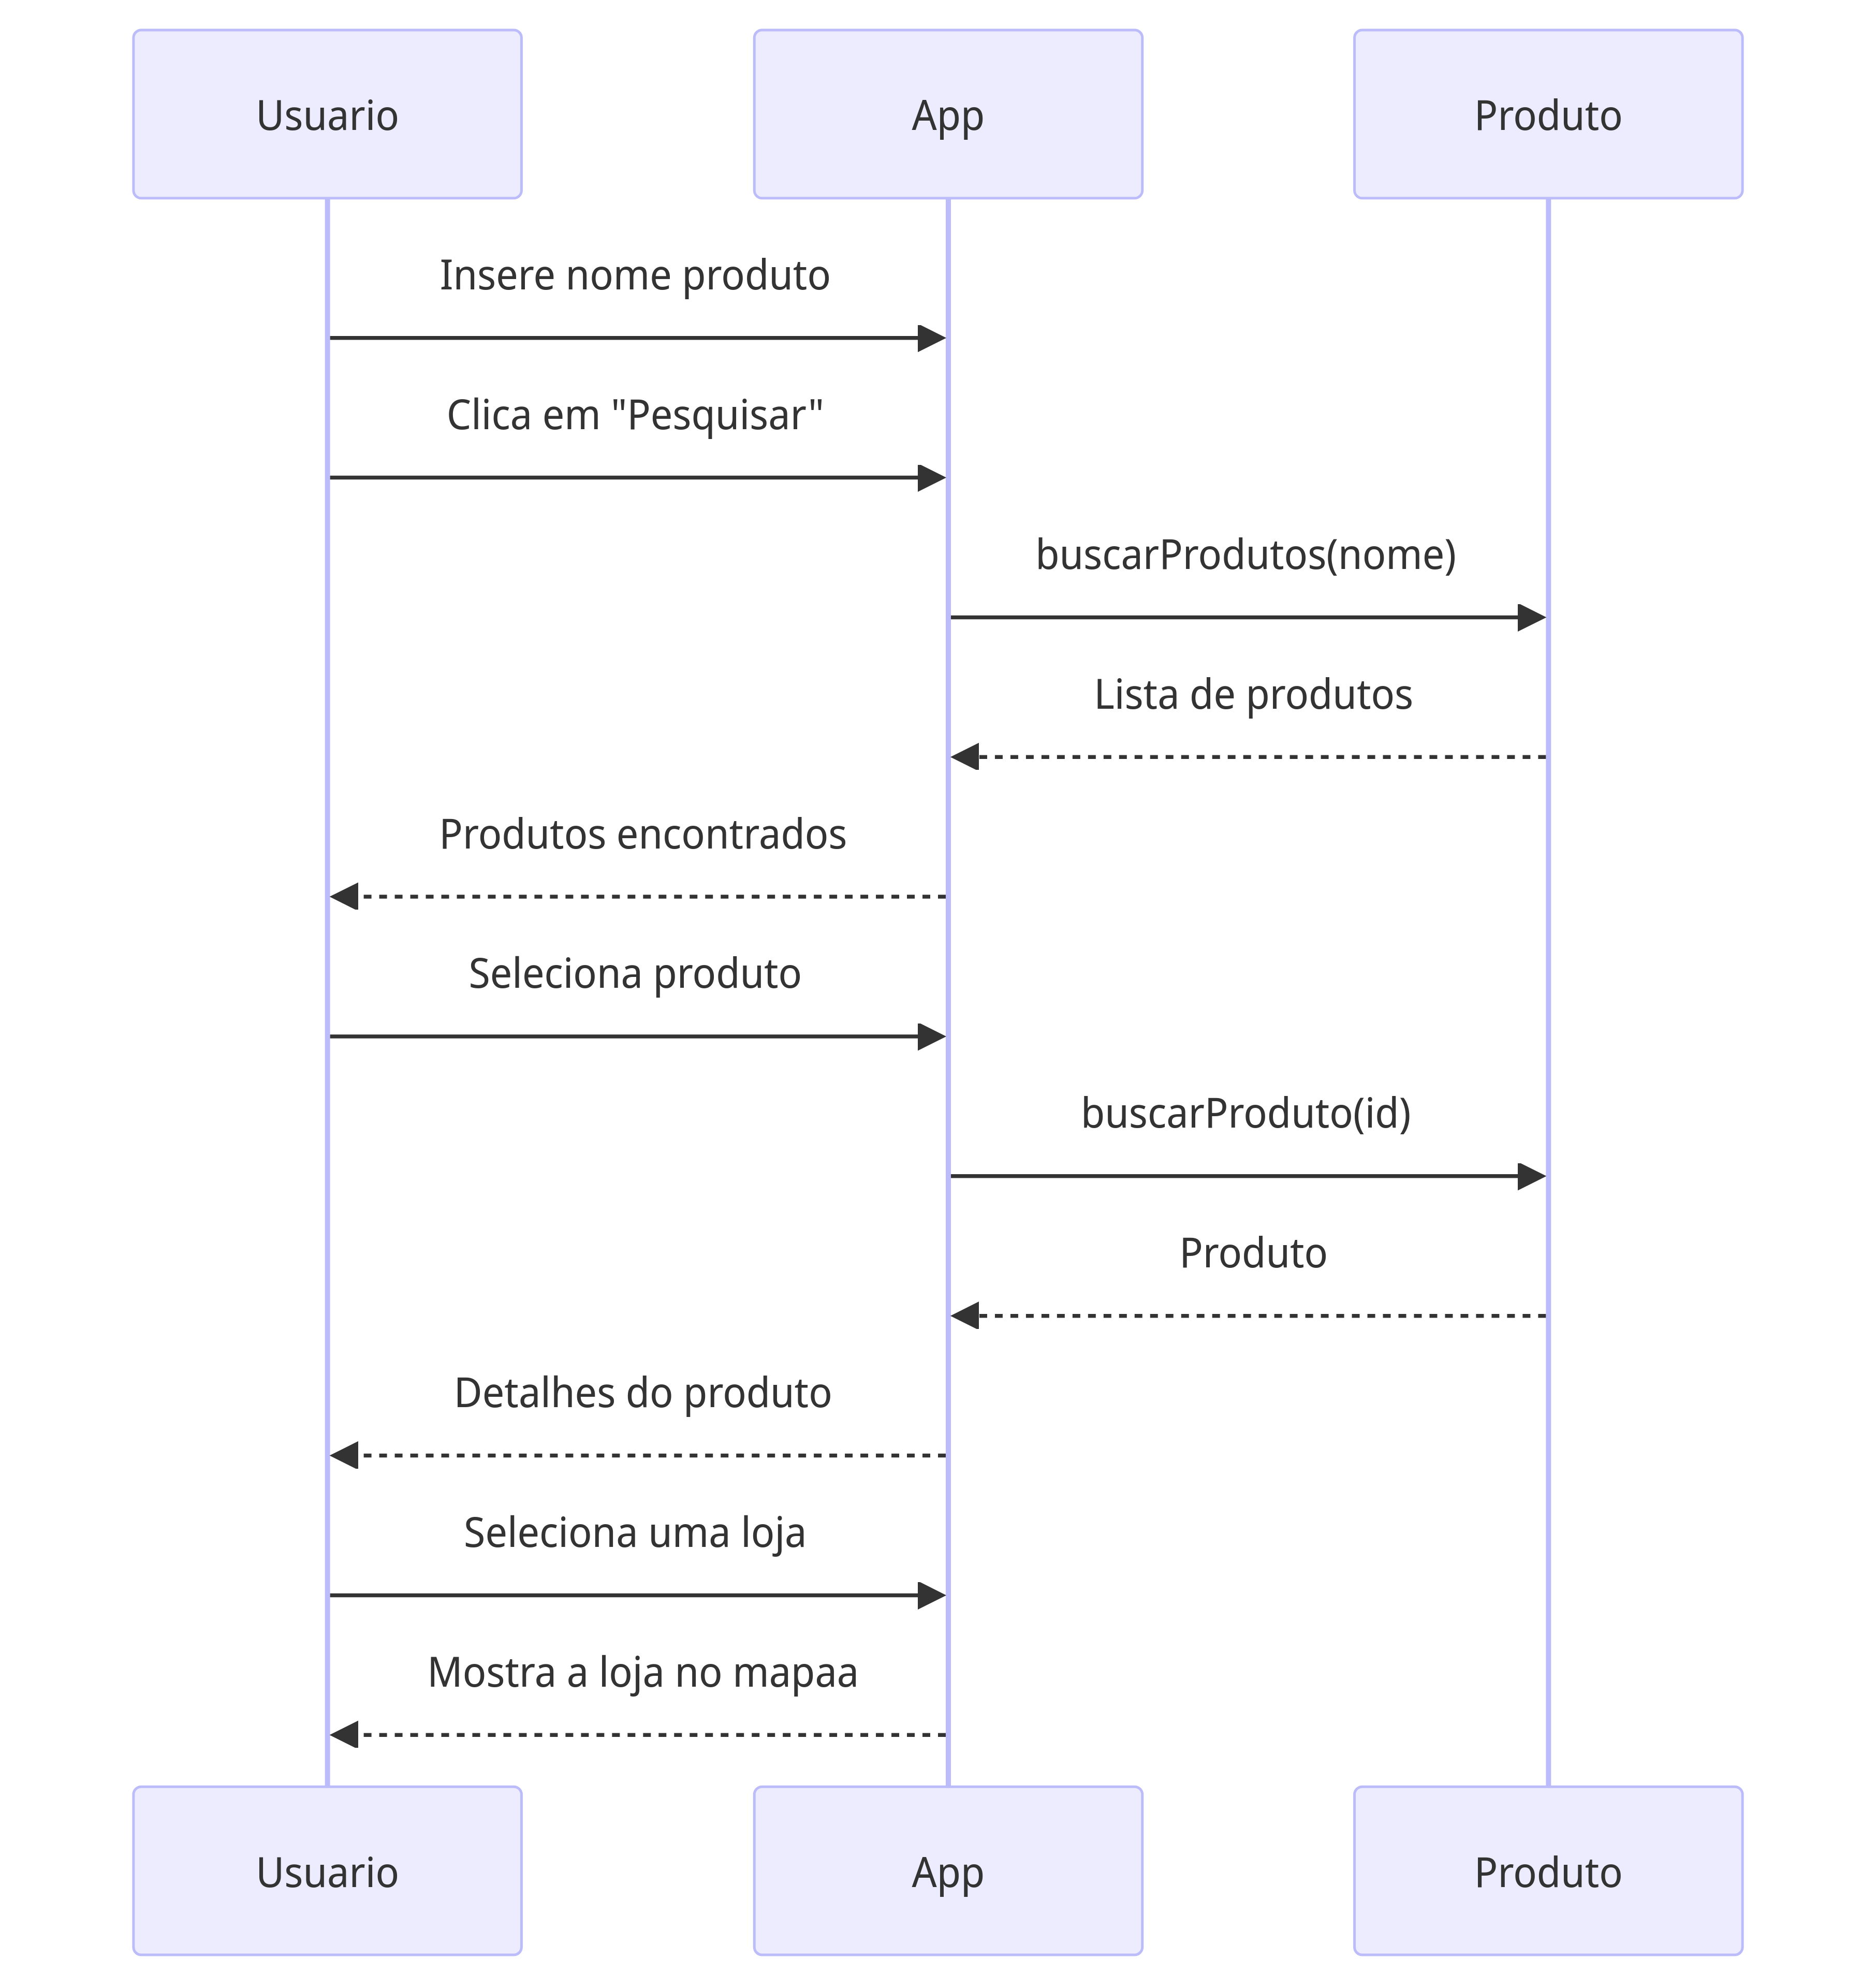
\includegraphics[width = 140mm]{fig/sequencia/sequencia1.png}
    \footnotesize \centering
    \par FONTE: O Autor (2024)
\end{figure}

\pagebreak 
\section{Cadastrar produto}
\begin{figure}[H]
    \caption{\label{fig:seqcadprod} DIAGRAMA DE SEQUÊNCIA CADASTRAR PRODUTO}
    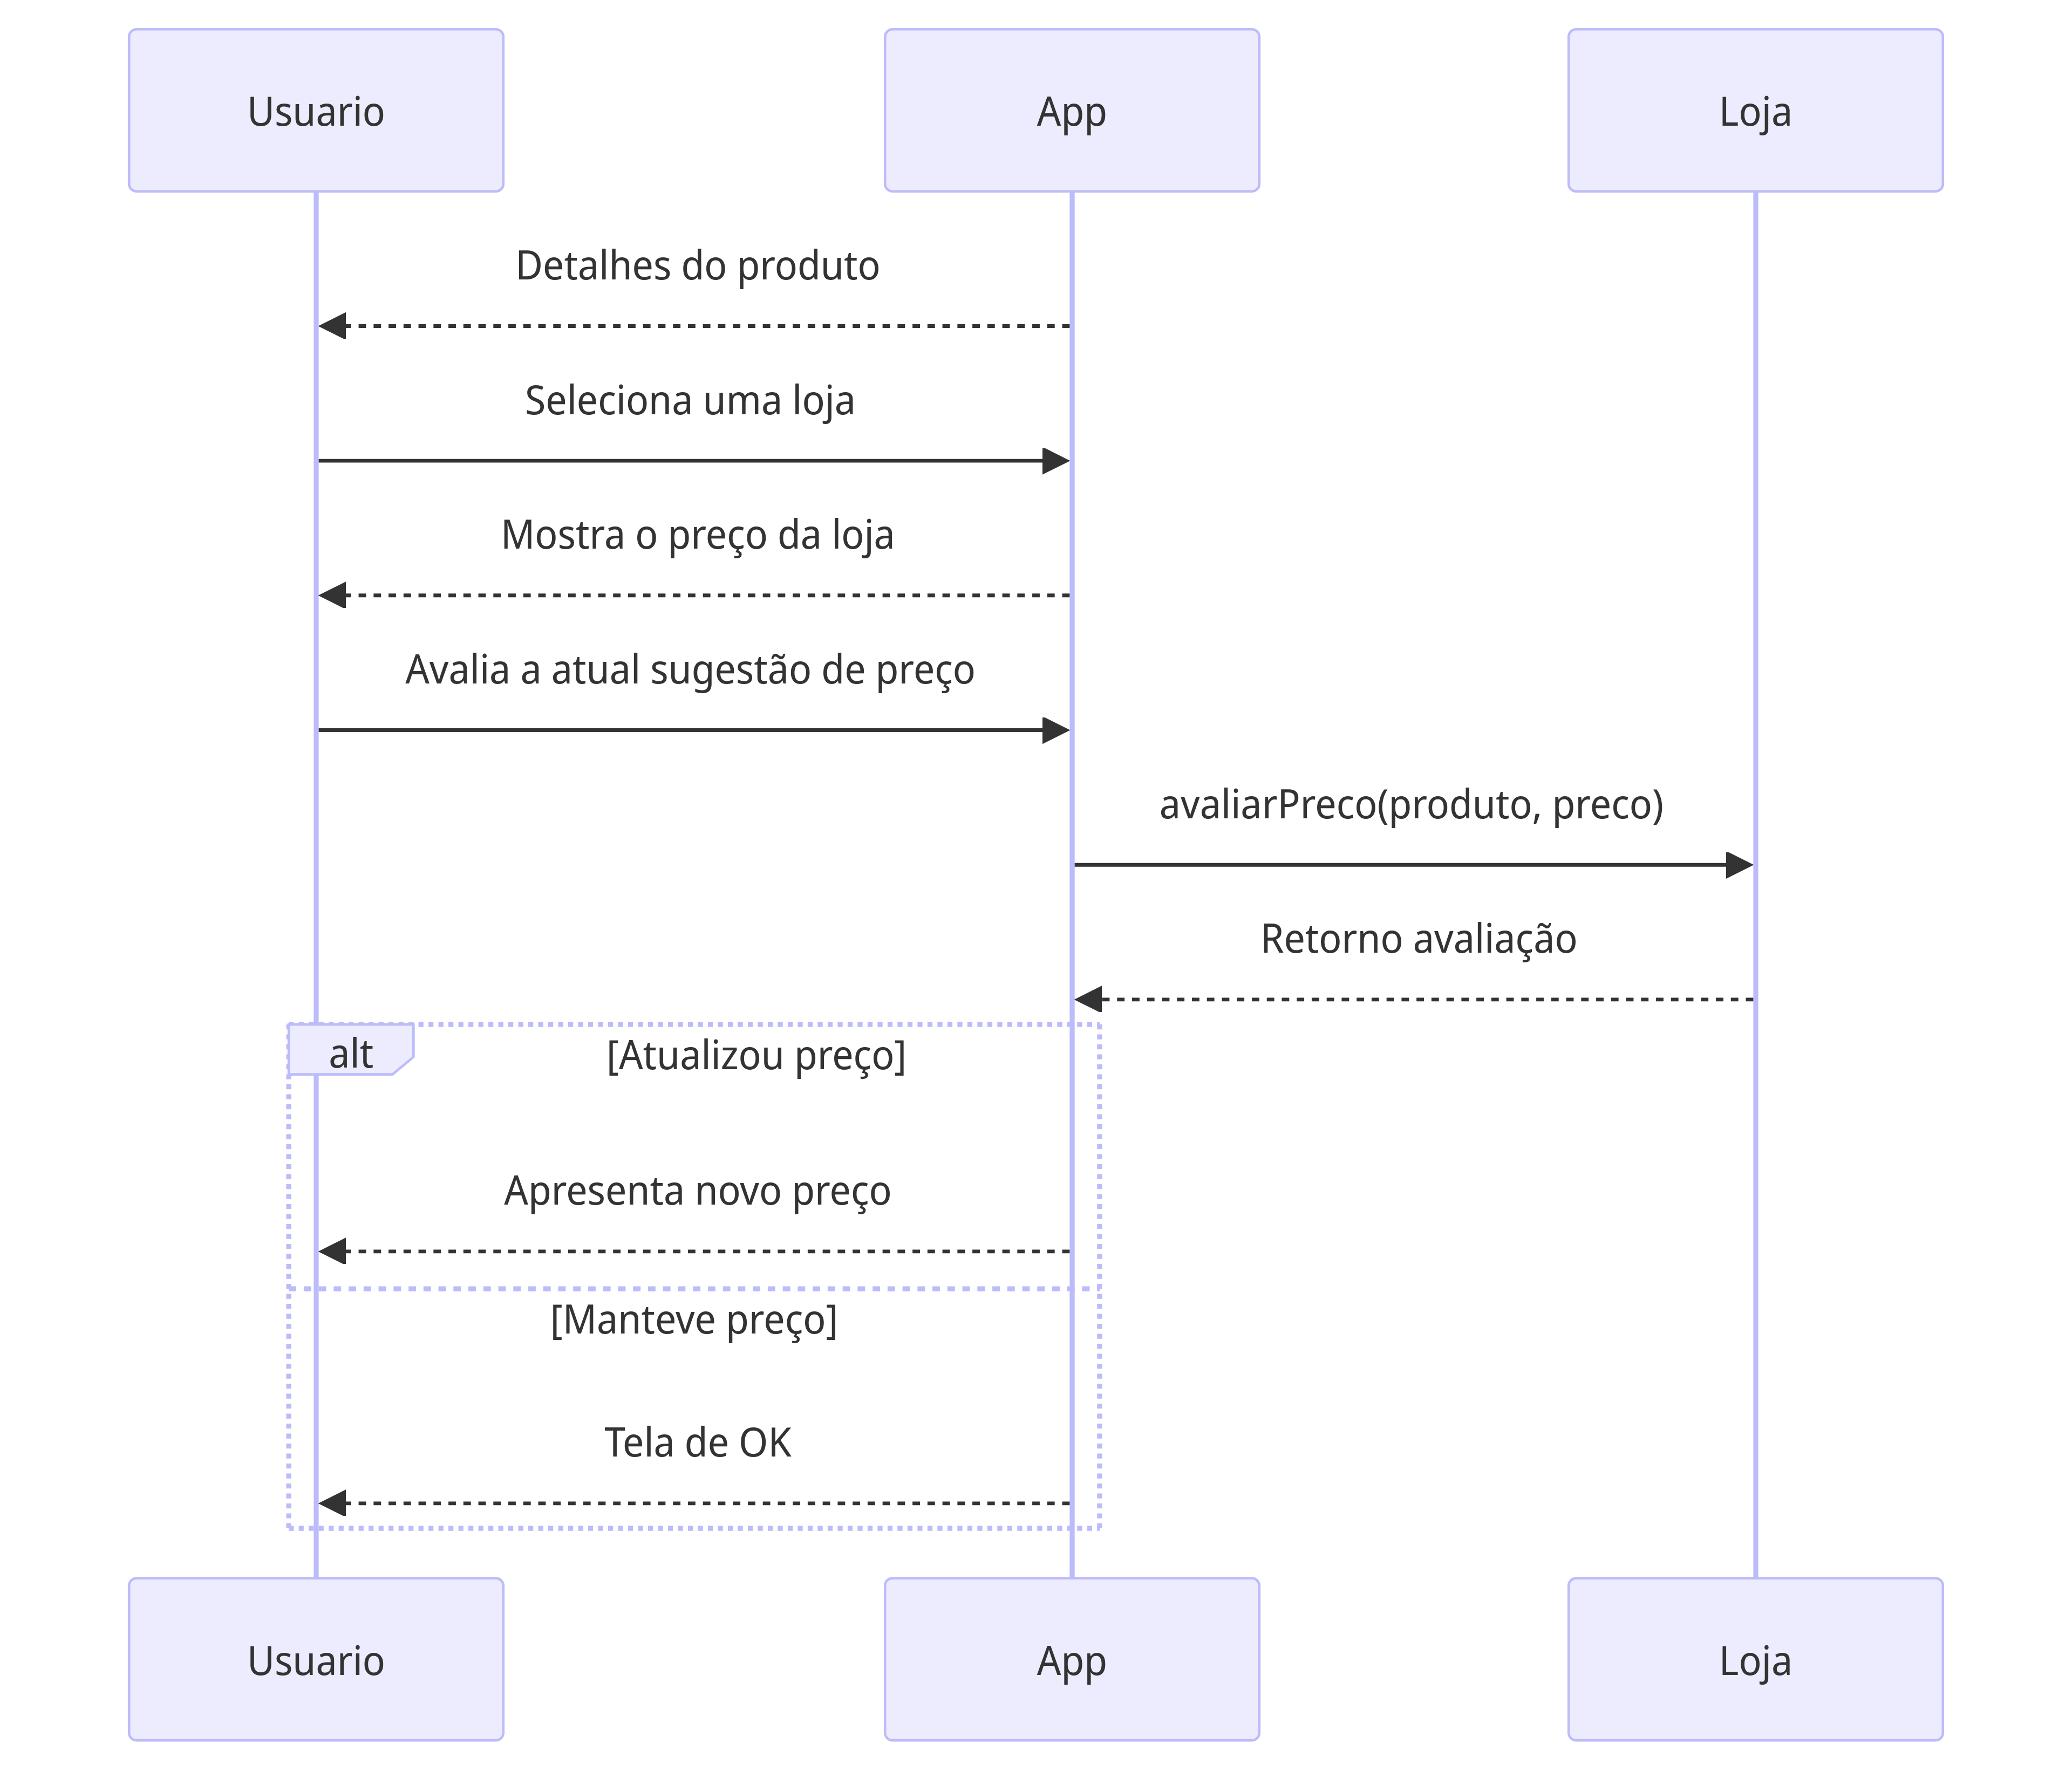
\includegraphics[width = 110mm]{fig/sequencia/sequencia2.png}
    \footnotesize \centering
    \par FONTE: O Autor (2024)
\end{figure}


\section{Avaliar sugestão}
\begin{figure}[H]
    \caption{\label{fig:label} DIAGRAMA DE SEQUÊNCIA AVALIAR SUGESTAO}
    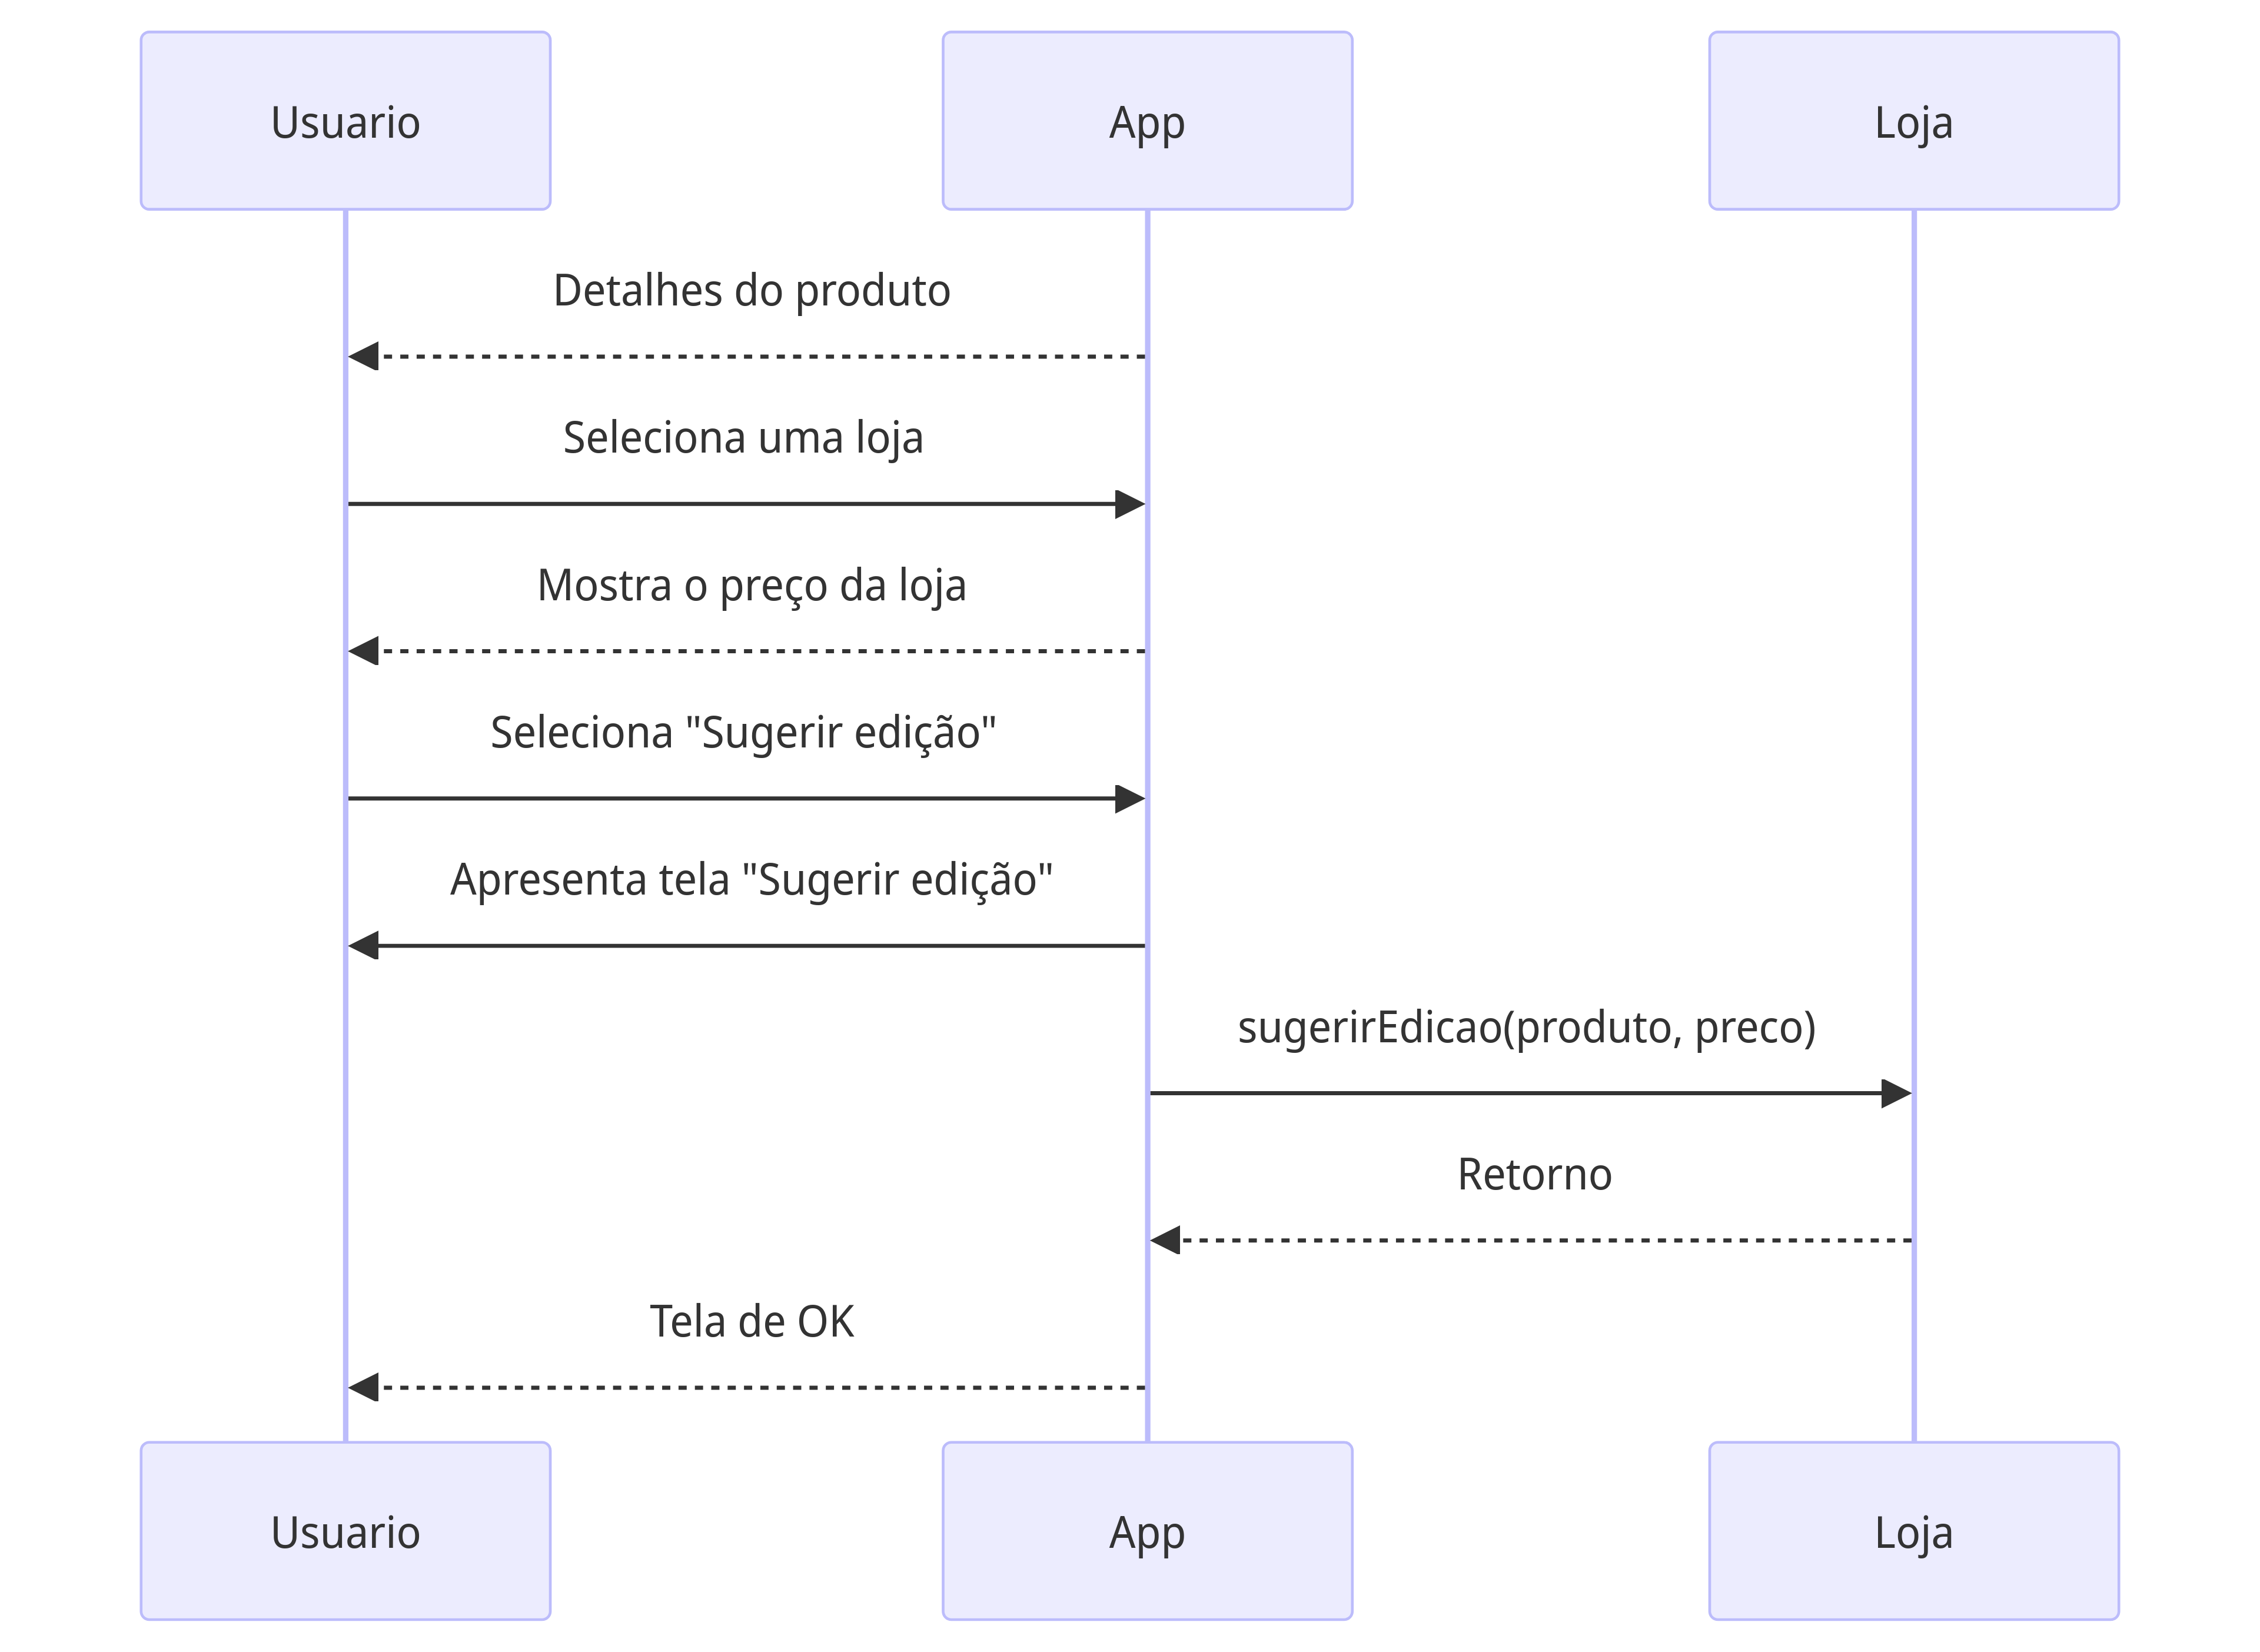
\includegraphics[width = 150mm]{fig/sequencia/sequencia3.png}
    \footnotesize \centering
    \par FONTE: O Autor (2024)
\end{figure}


\section{Cadastrar alerta}
\begin{figure}[H]
    \caption{\label{fig:label} DIAGRAMA DE SEQUÊNCIA CADASTRAR ALERTA}
    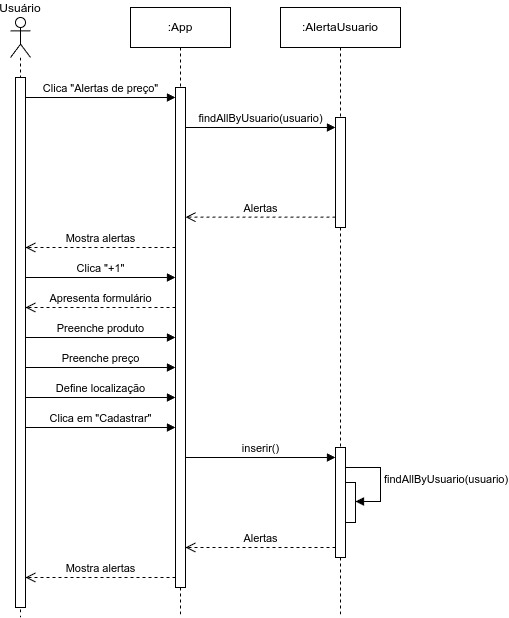
\includegraphics[width = 150mm]{fig/sequencia/sequencia4.png}
    \footnotesize \centering
    \par FONTE: O Autor (2024)
\end{figure}

%\section{Alterar senha}


%\section{Adicionar produto favorito}


%\section{Logar no sistema}


%\section{Criar conta}


%\section{Recuperar senha}